\subsection{Análisis de costos del proyecto}

En esta sección se presenta el desglose de los costos del proyecto. Con el propósito de facilitar el análisis de los gastos, estos se agruparon en diferentes apartados. Los rubros considerados son los siguientes:
\begin{itemize}
    \item Componentes mecánicos \ref{tab:mec_cost}. Principalmente se tiene en cuenta los elementos de transmisión de movimiento, motores y los elementos del sistema de trituración.
    \item Tornillería \ref{tab:tornillo_cost}. Todos los tornillos, rondanas y tuercas que se utilizaron para el prototipo.
    \item Componentes electrónicos \ref{tab:electronicos_cost}. Circuitos y elementos electrónicos del sistema.
    \item Componentes eléctricos \ref{tab:elect_cost}. Cables, fuentes y contactores.
    \item Materiales \ref{tab:mat_cost}. Se enlistan los perfiles, fibras, varillas y placas que se utilizaron.
    \item Consumibles \ref{tab:consu_cost}. Son todos los elementos que se utilizaron en el dispositivo y se fueron agotando.
    \item Herramientas \ref{tab:herra_cost}. Todos las herramientas o accesorios que se compraron para la elaboración del prototipo.
    \item Mano de Obra externa \ref{tab:man_ob_cost}. Servicios de manufactura externa e impresión 3D.
\end{itemize}


\begin{table}
    \centering
    \begin{tabular}{|c|c|c|} \hline 
         Cantidad&  Componente& Precio\\ \hline 
 1 pz& Molino de carne&919\\ \hline 
 2 pz& Chumaceras&310\\ \hline 
 1 pz& Motor de lavadora&800\\ \hline 
 1 pz& Riel din&160\\ \hline 
 10 m& Cinta de acero galvanizada&340\\ \hline 
 1 pz& Motor de 1/4 HP&3000\\ \hline 
 1 pz& Motorreductor&3000\\ \hline 
         1 pz&  Banda 3V 50 in& 114\\ \hline 
         1 pz&  Banda 3V 53 in& 162\\ \hline 
         2 pz&  Polea 2.5 in& 70\\ \hline 
         1 pz&  Polea 12 in& 250\\ \hline 
         1 pz&  Polea 14 in& 295\\ \hline 
         &  Remaches& 35\\ \hline 
         2 pz&  Portacandados& 50\\ \hline 
         2 pz&  Cinturones& 350\\ \hline 
         \multicolumn{2}{|c|}{Total}& 9855\\ \hline
    \end{tabular}
    \caption{Cotos de elementos mecánicos}
    \label{tab:mec_cost}
\end{table}

  \begin{table}
    \centering
    \begin{tabular}{|c|c|c|} \hline 
         Cantidad&  Componente& Precio\\ \hline 
 4& Tornillos 1/2" x 4"&92\\ \hline 
 4& Rondanas de seguridad 1/2"&16\\ \hline 
 4& Tuercas 1/2"&28\\ \hline 
 4& Tornillos 3/8" x 4"&36\\ \hline 
 4& Tornillos 3/8" x 3.5"&32\\ \hline 
 8& Rondanas de seguridad 3/8"&24\\ \hline 
 8& Tuercas 3/8"&40\\ \hline 
         16&  Tornillos 3/16"& 48\\ \hline 
         16&  Rondanas 3/16"& 16\\ \hline 
         16&  Tuercas 3/16& 16\\ \hline 
         \multicolumn{2}{|c|}{Total}& 348\\\hline
    \end{tabular}
    \caption{Cotos de la tornillería}
    \label{tab:tornillo_cost}
\end{table}
\begin{table}
    \centering
    \begin{tabular}{|c|c|c|} \hline 
         Cantidad&  Componente& Precio\\ \hline 
 1& ESP32&140\\ \hline 
 1& LCD 20X4&140\\ \hline 
 1& Modulo I2C&40\\ \hline 
 1& Sensor DHT11&40\\ \hline 
 1& Sensor DS18B20&45\\ \hline 
 1& Transistor TIP41&30\\ \hline 
 4& Resistencias 4.7 k &5\\ \hline 
         4&  Resistencias 1k& 5\\ \hline 
         5&  Botones con flex& 70\\ \hline 
         1&  Fuente 12 v& 150\\ \hline 
         1&  Adaptador de fuente de 12 V& 48\\ \hline 
         1&  Gabinete de interfaz& 80\\ \hline 
         16&  Tornillos plasticos& 64\\ \hline 
         1&  Pila de reloj& 8\\ \hline 
         1&  Modulo RTC& 100\\
 1& Jumper&70\\
 1& Ventilador&60\\
 2& Miniprotoboard&100\\\hline \hline 
         \multicolumn{2}{|c|}{Total}& 1245\\ \hline
    \end{tabular}
    \caption{Cotos de elementos electrónicos}
    \label{tab:electronicos_cost}
\end{table}

\begin{table}
    \centering
    \begin{tabular}{|c|c|c|} \hline 
         Cantidad&  Componente& Precio\\ \hline 
 5& Clavijas&150\\ \hline 
 1& Calentador&973\\ \hline 
 1& Multicontacto industrial&700\\ \hline 
 1& Contactor de 110 V a 25 A&200\\ \hline 
 1& Contactor de bobina&300\\ \hline 
 1& Fuente 24 V&200\\ \hline 
 1& Botonera&90\\ \hline 
         1&  Enchufe& 24\\ \hline 
         8&  Cable duplex& 82\\ \hline 
         6&  Cable de uso rudo de 3 hilos& 138\\ \hline 
         1&  Paquete de zinchos& 80\\ \hline 
         \multicolumn{2}{|c|}{Total}& 2937\\ \hline
    \end{tabular}
    \caption{Cotos de elementos eléctricos}
    \label{tab:elect_cost}
\end{table}

\begin{table}
    \centering
    \begin{tabular}{|c|c|c|} \hline 
         Cantidad&  Componente& Precio\\ \hline 
 1& Eje de acero 1 1/2" x 1 m&400\\ \hline 
 3& palas&200\\ \hline 
 1& Lamina pastica&1100\\ \hline 
 6& Varillas&700\\ \hline 
 1& Fibra de vidrio 2m x 1.2m&500\\ \hline 
 4& PTR 2x2 calibre 14 x 6 m&2000\\ \hline 
 1& Filtro de carbon activado&1150\\ \hline 
         2&  Codos de PVC de 45°& 50\\ \hline 
         1&  Tubo de PVC de 3" x 1m& 65\\ \hline 
         1&   Tambo de lamina& 200\\ \hline 
         \multicolumn{2}{|c|}{Total}& 6365\\ \hline
    \end{tabular}
    \caption{Cotos de materiales}
    \label{tab:mat_cost}
\end{table}

\begin{table}
    \centering
    \begin{tabular}{|c|c|c|} \hline 
         Cantidad&  Componente& Precio\\ \hline 
 2& Tiner botella 1 L&106\\ \hline 
 1& Bote pintura negra 1 L&250\\ \hline 
 1& Bote pintura roja 1 L&250\\ \hline 
 1& Paquete de estopa&50\\ \hline 
 1& Botella de removedor de pintura de 960 ml&180\\ \hline 
 1& Paquete de electrodos para soldar &100\\ \hline 
 2& Cinta de aislar &20\\ \hline 
         1&  Pegamento para PVC& 36\\ \hline 
         1&  Cinta teflon& 15\\ \hline 
         1&  Paquete de cubrebocas& 80\\ \hline 
         1&  Paquete de guantes de latex& 106\\ \hline 
         \multicolumn{2}{|c|}{Total}& \\ \hline
    \end{tabular}
    \caption{Cotos de elementos consumibles}
    \label{tab:consu_cost}
\end{table}

\begin{table}
    \centering
    \begin{tabular}{|c|c|c|} \hline 
         Cantidad&  Componente& Precio\\ \hline 
 2& Brochas&70\\ \hline 
 1& Cutter&15\\ \hline 
 4& Botes de 20 L&300\\ \hline 
 1& Disco de corte para metal&50\\ \hline 
 1& Disco de desvaste para esmeril&30\\ \hline 
 1& Broca 3/16&80\\ \hline 
         \multicolumn{2}{|c|}{Total}& 545\\ \hline
    \end{tabular}
    \caption{Cotos de Herramientas}
    \label{tab:herra_cost}
\end{table}

\begin{table}
    \centering
    \begin{tabular}{|c|c|} \hline 
           Componente& Precio\\ \hline 
  Soldadura de la base&4000\\ \hline 
  Pieza para el filtro&400\\ \hline 
  Adaptador de trituración&250\\ \hline 
  Sosten de ventilador&100\\ \hline 
  Adaptador a la entrada de materia&250\\ \hline 
         Total& 5000\\ \hline
    \end{tabular}
    \caption{Cotos de mano de obra externa}
    \label{tab:man_ob_cost}
\end{table}

Ahora se realiza la suma total de los valores descritos en las tablas, por lo que se obtiene un costo tal que se muestra en la tabla \ref{tab:gastototal}

\begin{table}
    \centering
    \begin{tabular}{|c|c|} \hline 
           Componentes mecanicos& 9855\\ \hline 
  Componentes eletronicos&1245\\ \hline 
  Componentes electricos&2937\\ \hline 
  Tornilleria&348\\ \hline 
  Materiales&6365\\ \hline 
  Consumibles&1193\\ \hline 
 Mano de obra&5000\\ \hline 
 Herramientas&545\\\hline \hline 
         Total& 27488\\ \hline
    \end{tabular}
    \caption{Cotos totales del proyecto}
    \label{tab:gastototal}
\end{table}
A partir de los datos de la tabla \ref{tab:gastototal}, se puede obtener la gráfica de la ilustración \ref{fg:rep_gastos}, la cual muestra la distribución de los gastos del proyecto. En ella se observa que los materiales y los componentes mecánicos concentran la mayor parte de la inversión, al representar el 59\% del costo total del proyecto. Por otra parte, el gasto correspondiente a herramientas y accesorios fue mínimo, debido al apoyo brindado por el laboratorio de Trabajo Terminal.
\begin{figure}[h!]
    \centering
        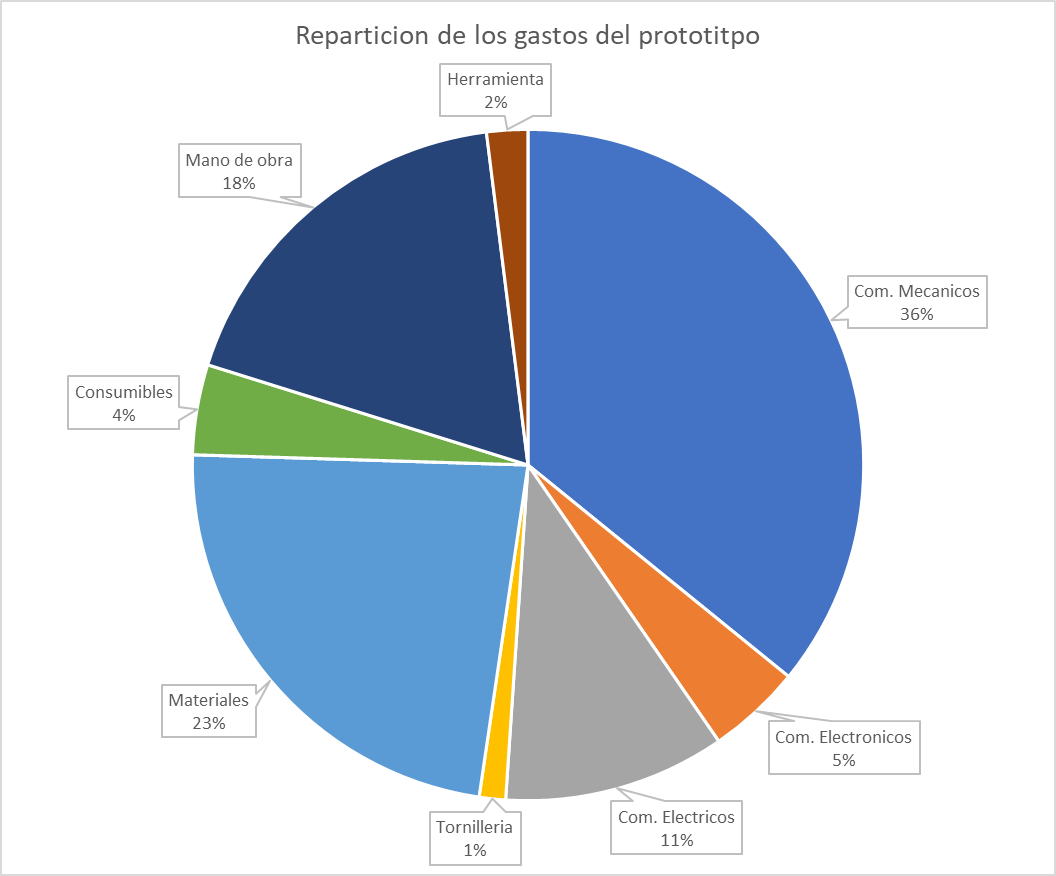
\includegraphics[scale=0.4]{images/Anexo/Reparticion_gastos.png}
        \caption{Repartición de los gastos}
    \label{fg:rep_gastos}
\end{figure}

\clearpage